%%%%% Document Setup %%%%%%%%

\documentclass[10pt,twocolumn]{revtex4}    % Font size (10,11 or 12pt) and column number (one or two).


\usepackage{times}                          % Times New Roman font type
 \usepackage{gensymb}
\usepackage{ragged2e}


\usepackage{CJKutf8} %Use of Japanese 


\usepackage[a4paper, left=1.85cm, right=1.85cm,top=1.85cm, bottom=1.85cm]{geometry}       % Defines paper size and margin length

\usepackage{physics}

\usepackage[font=small, labelfont=bf]{caption}    % Defines caption font size as 9pt and caption title bolded

%\usepackage[sorting=none]{biblatex}
%\addbibresource{refs.bib}
\usepackage{natbib}
\bibpunct{(}{)}{;}{a}{}{,} % to follow the A&A style


\newcommand*{\wasyfamily}{\fontencoding{U}\fontfamily{wasy}\selectfont}
\newcommand*{\astrosun}{{\odot}}
\newcommand*{\mercury}{{\text{\wasyfamily\char39}}}
\newcommand*{\venus}{{\text{\wasyfamily\char25}}}
\newcommand*{\earth}{{\oplus}}
\newcommand*{\mars}{{\text{\wasyfamily\char26}}}
\newcommand*{\jupiter}{{\text{\wasyfamily\char88}}}
\newcommand*{\saturn}{{\text{\wasyfamily\char89}}}
\newcommand*{\uranus}{{\text{\wasyfamily\char90}}}
\newcommand*{\neptune}{{\text{\wasyfamily\char91}}}
\newcommand*{\pluto}{{\text{\wasyfamily\char92}}}
\newcommand{\EST}{\angle_{\earth\astrosun a}}


\newcommand{\refeq}[1]{\textbf{Eq.#1}}
\newcommand{\reffig}[1]{\textbf{Fig.#1}}
\newcommand{\reftab}[1]{\textbf{Tab.#1}}
\newcommand{\refsec}[1]{\textbf{Sec. #1}}
\newcommand{\xsqrd}{\chi^2}
\newcommand{\E}[1]{\times10^{#1}}
\newcommand{\rem}{r_{\earth,w}}
\newcommand{\rsm}{r_{\astrosun,w}}
\newcommand{\err}[1]{\alpha_{#1}}


\usepackage{graphics,graphicx,epsfig,ulem}	% Makes sure all graphics works
\usepackage{amsmath} 						% Adds mathematical features for equations

\usepackage{etoolbox}  
\usepackage{amssymb}   
 % Customise date to preferred format

\makeatletter
\patchcmd{\frontmatter@RRAP@format}{(}{}{}{}
\patchcmd{\frontmatter@RRAP@format}{)}{}{}{}
\renewcommand\Dated@name{}
\makeatother

\usepackage{fancyhdr}
\usepackage{hyperref}

\pagestyle{fancy}                           % Insert header
\renewcommand{\headrulewidth}{0pt}
\lhead{J. K. Read}                          % Your name
\rhead{}            % Your report title               

\def\bibsection{\section*{References}}        % Position reference section correctly


%%%%% Document %%%%% 
\begin{document}

\title{Mitaka's Minability: A Review of how Lightcurve Analysis Can Be Used to Find Mineable Asteroids} 
\date{Submitted: \today{}, Observational Per: January, 2023 to March 2023}
\author{Read, J. K. (and Lund, M.)}
\affiliation{\normalfont Astrolabs 2023: Epiphany}



\begin{abstract}    
Asteroid mining is an exciting possible method with which to gain access to new materials for human use, on and off of Earth. Minerals valuable on Earth may be able to be found in larger quantities on asteroids and sent back to Earth by private companies, however the introduction of this new material will inevitably cause a drop in the price of any minerals brought to Earth to the large influx of yet before unreachable sources. Another possibility is to use the material mined off of asteroids in-situ to create more mining craft in space, and create the beginnings of human civilisation away from Earth. 1088 Mitaka was observed in order to test a simpler method of screening asteroids as mining candidates than using high resolution imaging that may require satellites. By observing the variance of the brightness of Mitaka in time, and lightcurve (LC) can be formed, and by analysing the LC the period of Mitaka can be found, $P_w = 0.1264707842 \pm 1\times10^{-10}days$. Then using the LC and the period, a convex hull can be modelled by fitting the LC of the model to that of Mitaka. The shape of Mitaka can be assessed for its appropriateness for mining. Then the material area of two cross-sections of Mitaka can be found $A_\alpha=(300 \pm 60)\times10^6 m^2$ and $A_\Omega = (500\pm 600)\times10^6 m^2$. The volume can then be approximated from the calculated areas $V_w = 8000 \pm 13100 Km^3$, and by comparison to the average density of other S-types,$\rho_S = 3000 \pm 900 Kg m^{-3}$, the mass can be approximated $m_w = (2 \pm 4)\times10^{13} Kg$. Lastly, by comparison to the average fractional mass of minerals in S-types, $Z$, the approximate amount of a mineral in Mitaka can be found, e.g. $m^w_{Fe,Ni} = (7\pm10)\E{12} Kg$.
\end{abstract}

\maketitle

\thispagestyle{plain} % produces page number for front page

\section{Introduction}

Asteroid mining is the process of extracting minerals from asteroids and either using them in-situ or returning them to Earth in order to use the materials for on-world purposes. The idea has gained more attention as private space companies start their own explorations into space for the means of earning revenue rather, or at least more importantly than, scientific exploration. 
The vast amount of resources that are theoretically extractable from asteroids cover a wide range of economic areas. Precious metals such as gold and platinum can be brought to Earth for use in what would almost definitely be called "space jewellery" and sold for millions of dollars, or used for making electronics both on and off-world. Iron and Nickle are vital ingredients in the creation of steel, so would be very useful both in making more structures on Earth or making more space-mining equipment in space to extract ever more material. Water may also be able to be made from the material present on asteroids, and hydrogen may even be used in power cells to power the whole operation with no refuelling from Earth. 
It is clear to see then the possibilities in asteroid mining invite a host of new avenues for monetary gain for companies that can achieve the feat. However, the addition of these never-before-available resources to the economy of Earth would cause a reactionary reduction in price. As the present work is not a review of the economics of mining asteroids, this topic will be avoided, and the bulk of discussion will be on the in-situ uses of the minerals available to mining operations, manned and unmanned.  
The challenges latent in asteroid mining before any mining rig has even landed are the assessment of candidates for mining asteroids. To assess which asteroids are good candidates, the shape and composition of the asteroid are the two most important factors. 
The shape is important as the stability of the asteroid while mass is being removed is vital in how complex the mining operation will be. An asteroid with a shape that makes as much of its surface easily accessible will be the best candidate as the machinery necessary to traverse it can be simpler and therefore cheaper.
The composition of the asteroid is just as important as an asteroid with more valuable minerals will obviously be more worthwhile to mine.
So the best mining candidate, for in-situ purposes, then is an asteroid that has an easily transversal shape that has a stable centre-of-gravity, that also has many valuable resources that can be used in construction and the creation of more mining and propulsion equipment to spread the mining operation to more asteroids. 

Asteroids are most often non-spherical and rotate about an axis while orbiting the Sun, $\astrosun$. This means different cross-sectional areas of the asteroid, $A^a_i$, will be facing Earth, $\earth$, throughout the rotation of the asteroid, each of which will reflect a differing amount of luminosity, $L$, from the sun onto Earth. Ground-based observations then can measure the varying brightness of the asteroid to form a curve of the brightness of the asteroid in time, called a lightcurve (LC), resultant from the rotation of the asteroid causing the change in cross-section facing Earth. As at some point the asteroid will complete a full revolution, the LC will be periodic with the same period as the asteroid, so the period of the LC can be found to find the rotational period of the asteroid.

By combining the data from several nights by comparing brightness to phase $\phi$ rather than time, the data from several nights can be used to fit a single lightcurve to the data in order to archive a lightcurve more representative of the asteroid. In doing this, a period can be found for the asteroid by minimising the spread of brightness for each phase, and as before the period of the LC is the period of the asteroid. The use of many observation sets is not only useful in finding an average to increase accuracy but also because after three weeks the target-Sun-Earth angle will have changed with some significance. This means the asteroid will be being observed from another side, so the composite lightcurve can then recover details of more orientations of the asteroid. 

This newly found fitted lightcurve and period can then be used to construct a model of the asteroid. This is done by finding a mathematically described model of a convex polyhedron, and processing its scattering to compare its lightcurve to that of the observed asteroid, and minimising the difference. This will result in a convex representation of a model of the asteroid. This can give an idea of the overall shape of the asteroid, but will obviously miss out smaller, non-structural details and curved details like craters and outcroppings. This shape can then be reviewed in order to determine if the asteroid is suitable to be investigated further as a mining candidate. 
The reason this more imprecise investigation is an important step for identifying mining candidates is the more detailed imagery or modelling of an asteroid is expensive and requires specialist equipment such as high-detail telescopes and cameras, mounted on high remote mountains or on satellites in space. Therefore even gaining a rough idea of the appropriateness of an asteroid from relatively simple equipment and image processing can be instrumental in not wasting time and money observing asteroids with the more specialist equipment that turn out to not be good for mining. 

In addition to finding the model of the asteroid, the composition can be found in order to assess if the asteroid contains sufficiently valuable material to be worth mining. Through comparison with how much flux is reflected from the asteroid and reaches Earth $f_\earth$ with the amount incident on it $f_a$ by two different faces, a simple parallelogram-faced prism can be constructed to approximate the volume of the asteroid. After this, assuming the asteroid has similar density $\rho$ and composition to others of the same class $\rho_{class}$, the mass $m_a$ and amount of minerals in the asteroid can be approximated to assess if an asteroid is a good candidate for mining.
As the focus here is on possible in-situ uses of material, an asteroid rich in metallic material useful in the construction of buildings and new craft, as well as elements useful in the creation of power and power storage than could power more mining craft or possible human habitations, would be the optimal candidate. 

Overall then, the aim is to identify an asteroid that has a good shape for transiting about the surface and will have a steady centre of gravity, which is done by modelling it as a convex hull. Then after this, approximate the mass by approximating the volume by constructing a parallelogram-faced prism by finding the area of two faces of the asteroid from observed brightness. The composition can then be estimated by comparison to other asteroids of the same class.  

\section{1088 Mitaka}
1088 Mitaka (prov. 1927 WA) is an asteroid in the inner region of the asteroid belt, with a semi-major axis of $a_w = 2.201288900683571\pm4.0712\times10^{-9}AU$ \cite{jplMitaka}. Mitaka is an S-type asteroid, meaning it contains silicate minerals such as pyroxenes. Mining and possibly processing these materials off-world is an attractive alternative as so-called tailings from the processing of these minerals can be toxic to Earth environments. S-type asteroids also contain metallic Iron-Nickle (Fe-Ni) minerals as well as Magnesium. Fe-Ni materials are used in the creation of stainless steel, and Mg is useful in the creation of lightweight alloys that are used in aerospace applications, but typically not in Earth-based spacecraft due to the possibility of fire at the high temperatures present in leaving Earth. Therefore the presence of these metals on Mitaka is attractive as it would allow for the creation of strong materials in-situ in space, and would mean that magnesium alloys could be used for craft as they would not have to withstand take off from Earth. Therefore the abundance of metallic and silica materials in S-type asteroids, and so theoretically Mitaka, would make it a good candidate for asteroid mining for the purpose of using the material in-situ. 

Mitaka was chosen to be observed as it was over $70^o$ from the horizon most of the night, on all nights it was to be observed. This is important as the closer an object is to zenith ($90^o$ above the horizon) have less atmosphere in front of them, which leads to less atmospheric disruption. It also allowed for observations on most nights to capture more than one rotational period. Mitaka being an S-type asteroid also means it is a relatively bright asteroid, with albedo $\varpi_w = 0.15 \pm 0.03$, so observing it on Earth is easier than say C or D-types.


\section{Observations} 
Two Telescopes were used: Draco-2, a remote access $14ft$ telescope, and East-16, with a $16ft$ mirror. Both have charge coupled devices (CCDs) in order to collect photons from objects to generate images. 

To focus the telescopes the CCD was moved further or closer to the telescope lens to minimise the effect of atmospheric turbulence via minimising seeing. The seeing was the full width at half maximum of the light diffusion, essentially the spreading out of the light that would otherwise look point-like with no atmosphere.

As the variation of brightness was observed, the clear, C, filter was used to allow in the most amount of light possible. To this end also, an exposure time of 30s was used to capture as much light from Mitaka as possible while still capturing many images during a night. 

So, the telescope was pointed at Mitaka using coordinates fetched from the JPL ephemeris database and then focused. A shutdown time is decided automatically by sensors detecting adverse conditions like wind and f temperature, or manually by selecting a number of exposures before shut off. $30s$ exposures were then taken of Mitaka over the observing period of that night. The observations of Mitaka were captured in early 2023 over 5 days: 17, 18, 20, 25 Jan and 13 Feb, a full log can be found in \textbf{Tab. \ref{tab:obsTable}}. Weather was typically clear, with seeing always about $3"$ due to atmospheric disruption after focusing, common in Durham. Mitaka was observed for over an entire period for all nights except 25 Jan, seen in \reffig{\ref{FastSolveAllEntire}}.

After observing Mitaka a night, the data are checked for outlier readings. There was a transit on 17 Jan and 18 Jan, the data of which were removed as the extra light caused an erroneously bright reading. Also, due to the lowering of the asteroid toward the horizon as the Sun approached the horizon, Mitaka seemed dimmer closer to dawn. Therefore, the 18 Jan lightcurve was split into approximately three periods of rotation, 18a, 18b, and 18c.

\subsection{Aperture photometry}\label{ssec:aperturePhotometry}
Aperture photometry is used to measure the brightness of objects, via measuring the total amount of light that falls within a circular aperture centred on the object in question. 
The aperture size is an important factor in measurement to get accurate results, an aperture too small will not capture all the light from an object, but too large will cause too much background to be included in the measurement. Therefore, the aperture size must be calibrated so that the ratio of signal-to-noise $S/N$ is maximised. The signal, $S$, is defined as the sum of counts in the aperture and the noise, $N$, is the counts from the background sky $B$ close to the object plus the signal, to account for noise in the aperture. The calibration is performed by placing an aperture over the object of some radius $r_{ap}$, and calculating $S/N$ using \textbf{Eq. \ref{eqn:S/N}}. This is done for many values of $r_{ap}$ and at the radius where $S/N$ peaks this will be the $r_{ap}$ used in following photometry. Maximising $S/N$ is important as a high $S/N$ indicates a reliable signal, whereas a low $S/N$ indicates a very noisy signal with high uncertainty. 

\begin{equation}\label{eqn:S/N}
    \frac{S}{N} = \frac{S}{\sqrt{S + B}}
\end{equation}


Observations from 20/01/2023 were used in the aperture photometry process, using the GAIA image display and analysis program. The aperture producing the best $r_{ap}$ was $3"$, seen in \textbf{Fig. \ref{fig:SMAPlot}}.

\begin{figure}
    \centering
    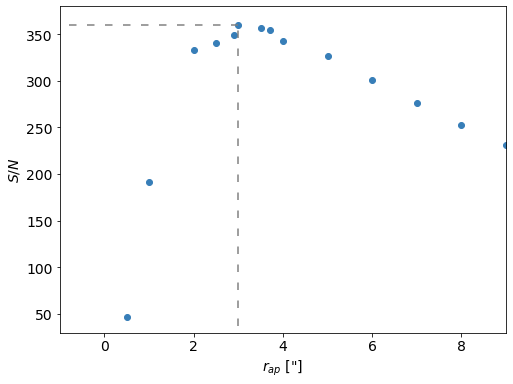
\includegraphics[width=\linewidth]{ApPhotoPlot.png}
    \caption{Plot of Signal-to-Noise, $S/N$, ratio by aperture radius $r_{ap}$ to determine best $r_{ap}$ to analyse observations. }
    \label{fig:SMAPlot}
\end{figure}

From here the magnitude of Mitaka, $M_w$ can be found in an image by placing an aperture of $3"$ around it in GAIA and reading off the total counts, then using,
The magnitude of an object from the counts is,
\begin{equation}\label{eqn:Mag}
    M = M_0 - 2.5\log{N},
\end{equation}
where $N$ is the number of counts, and $M_0$ is a zero-point.

A local python program called \textbf{aphot.py} was used to automate the process of calculating the magnitude of Mitaka in each image, from each observational session, using the calibrated aperture size of $3"$. This procedure was also carried out on two "calibration" stars, to be used to correct for atmospheric disruption. These magnitudes were then saved to a file called \textit{summary.obs}. Importantly, \textit{aphot.py} used a flat-field in order to correct for how imperfections on the telescope affected the magnitude results. A fixed zero point of 20 was also used as Mitaka was being examined for relative changes.  

Each night of observation had 2 calibration stars with, the right ascensions $\alpha_*$ and declinations $\delta_*$ of which can be seen in \reftab{\ref{tab:calStars}}.
\begin{table}[]
    \centering
    \begin{tabular}{c|c|c|c|c}
         Date &  $\alpha_1$ $[^o]$ & $\delta_1$ $[^o]$ & $\alpha_2$ $[^o]$ & $\delta_2$ $[^o]$ \\ \hline
         17 Jan & 104.770935    & 34.143249 & 104.591657 & 34.1097928 \\ 
         18 Jan & 104.4831      & 34.1033   & 104.3729 & 34.1644 \\
         20 Jan & 103.835       & 34.149    & 103.789 & 34.179 \\
         25 Jan & 102.6035      & 34.1999   & 102.5598  & 34.1479 \\
         13 Feb & 99.9078587    & 33.7723495 & 99.8072979 & 33.7816898 \\
    \end{tabular}
    \caption{Table showing the right ascension, $\alpha$, and declination, $\delta$ in degrees of the calibration stars used to perform differential photometry for each night.}
    \label{tab:calStars}
\end{table}

\subsection{Differential Photometry}\label{ssec:diffPhotometry}

Just measuring the brightness of an object can only go so far, as there are atmospheric disruptions can make readings brighter or dimmer, in Durham mostly dimmer. These disruptions must therefore be accounted for after aperture photometry is performed. 

Therefore, differential photometry is used to adjust the magnitude of the asteroid using comparisons to stars, as they are considered to be constant in brightness, to correct for the effect of atmospheric disruption, so any variation in brightness is due to the changing cross-section of the asteroid as it rotates, not atmospheric effects. 

Two stars are identified that do not saturate, are similar in brightness, and are close to the asteroid to use as calibration stars. This is so the atmosphere affects them in approximately the same way as the asteroid.

The process of adjusting the magnitude of the asteroid starts by assuming the magnitude of the stars from the initial image in a set $M_{init}^*$ of both stars is correct (this method is for relative adjustments so this will not lead to systematic error).

Then, for each reading of a star's magnitude from subsequent images $M_i^*$ find $\Delta M_i^* = M_{init}^* - M_i^*$. This creates a difference map for each star, $\{\Delta M^*\}$, which is a map of how to correct the magnitude readings of the star to account for atmospheric disturbance. These two maps are then averaged to create a correction mask, $\{\Delta M\}$ that accounts for atmospheric disruptions which is then added to the lightcurve of the asteroid.  
A local python program called \textbf{raw2dif.py} is used to compute this automatically over an entire set of observations. This is done automatically by giving in the \textit{summary.obs} from \textit{ahpot.py} to find the mask using the magnitudes of the two calibration stars saved, then applying it to the object magnitudes in the same file. The raw data and masks created for 17 Jan can be seen in \reffig{\ref{fig:mask}}.

\begin{figure*}
    \centering
    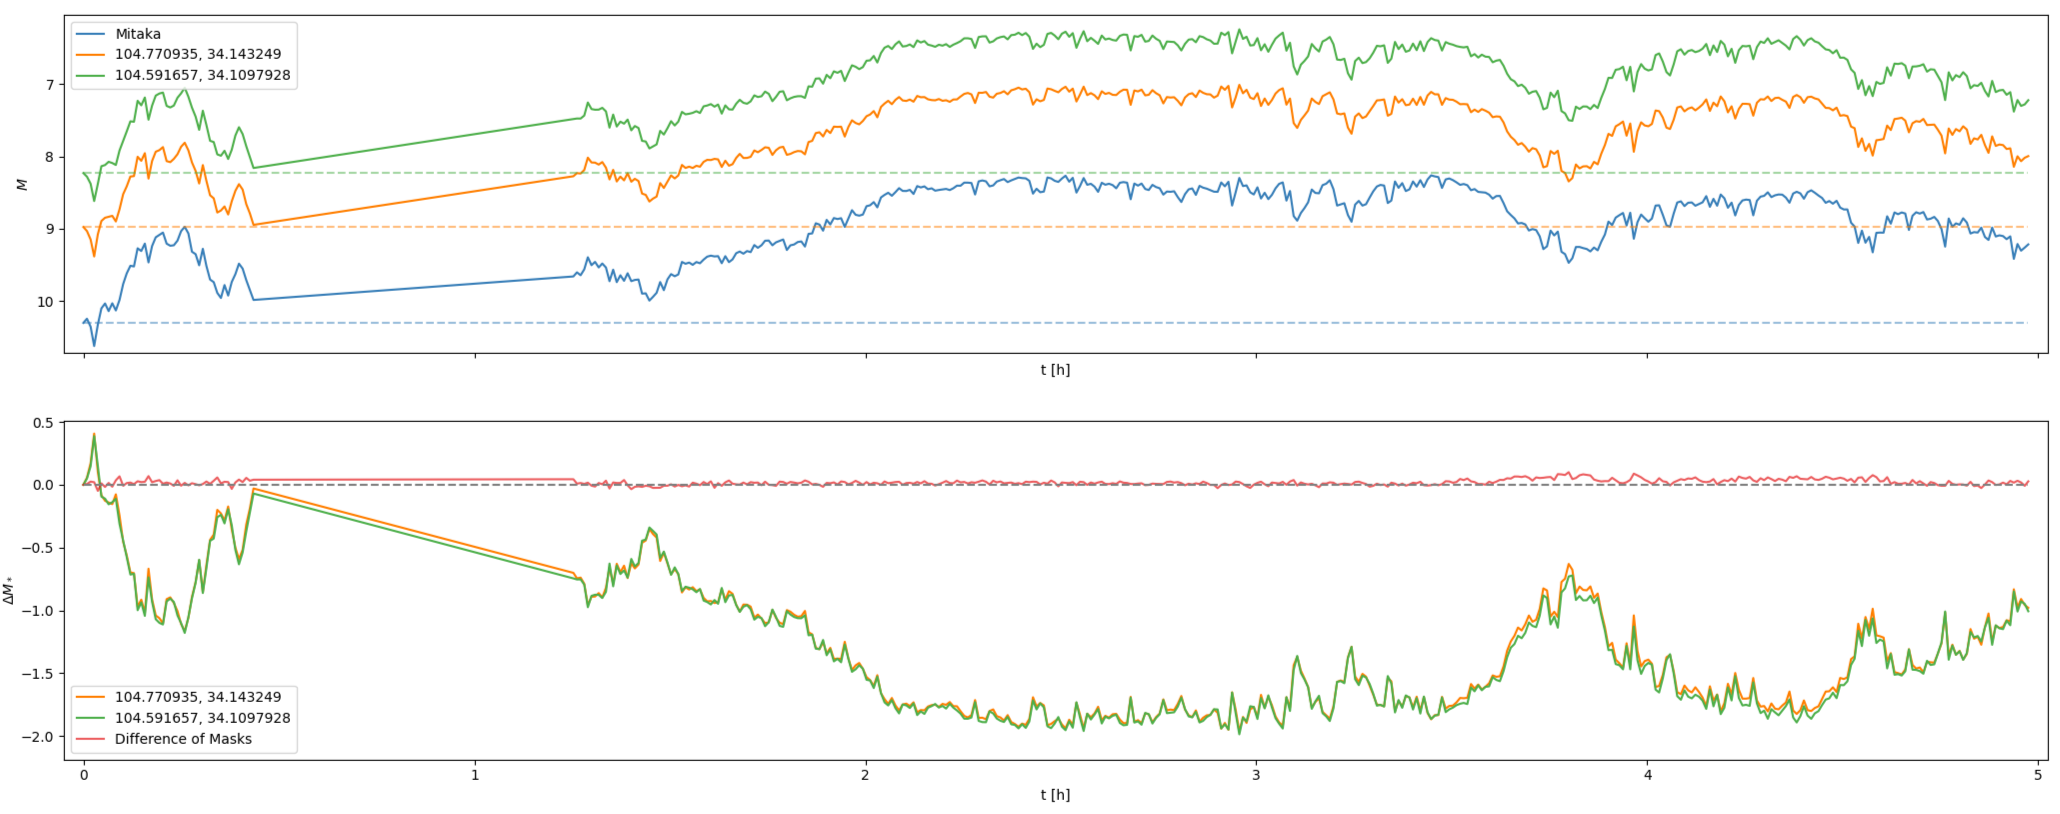
\includegraphics[width = \textwidth]{CalibrationMask.png}
    \caption{Above: the raw data collected from observing Mitaka, blue, and the two calibration stars used on 17 Jan, orange and green, by time. Below: The calibration mask created by finding the difference in the two stars initial magnitudes $M_0^*$ and the magnitude at time $t$ $M_i^*$. The difference in the two masks is shown in red. The large gap is due to the removal of data from when Mitaka was transiting a star.}
    \label{fig:mask}
\end{figure*}

\section{Finding the Period}\label{ssec:findP}

To find the rotational period of an asteroid, its lightcurves from different observations are compared. This "folding" is achieved by having each datum plotted against what phase of rotation $\phi$ it was recorded at rather than time, given some period $P$. To find the correct period, some $P$ is assumed and then each datum is assigned to a phase depending on when in this period $P$ it was measured. By finding the period with minimal spread of magnitudes in each phase $\delta M$, normalised by the error on them $\sigma M$, the correct period can be calculated.

To do this a local python program called \textit{fastsolve.py} is used as follows. The program is given an initial period $P_0$ and a percentage width about $P_0$ to create a set of periods to investigate ${P}$. It is also given how many phase bins, $N_b$ there should be, and which lightcurve files to read (the summary.obs files mentioned in \textbf{Sec. \ref{ssec:diffPhotometry}}). Then for each period $P_i \in {P}$ the program splits $P_i$ into $N_b$ phase bins of width $P_i/N_b$. Then each magnitude reading $M_k$ measured within the a phase in bin $b_j$ is placed in $b_j$. Then spread of all $M_k$s is calculated in each bin and summed to get $\Delta M$, and the best-fit period $P$ is the period at which $\Delta M/\sigma M$ is minimised.$\sigma M$ is the error on a given magnitude, and is used to normalise the spread. 

As the period is calculated using an algorithm applied to many combined data sets, the error on the period is found not via simple error propagation equations but through jackknife resampling, described in \refsec{\ref{ssec:jackknifing}}. 


Initially for Mitaka $P^w_0 = 0.126 days$ with the initial point if zero rotation set to 17 Jan 18:41. The set of periods swept through was $[0.12008, 0.13272]$ with bins $N_b = 10000$, for bin width $1.26\times10^{-6}$. Then after performing lightcurve folding using \textit{fastsolve.py}, show in \reffig{\ref{fig:findP}}, it was found Mitaka has a period $P_w = 0.1264707842 \pm 1\times10^{-10}days$, which is just over $3hr$.

\begin{figure}
    \centering
    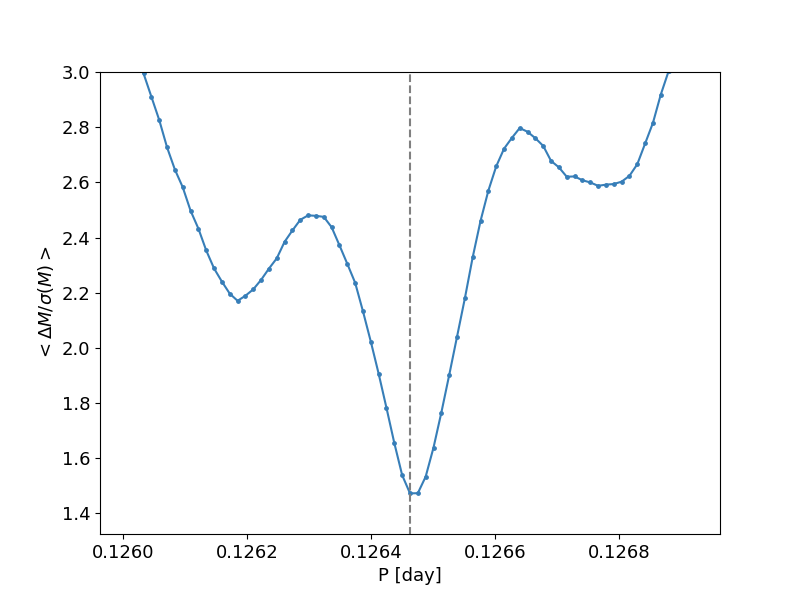
\includegraphics[width = \linewidth]{FastSolveAllPeriodZoomed.png}
    \caption{A plot of normalised magnitude spread $\Delta M/\sigma M$ by period $P$ to solve for the best-fit period of Mitaka, zoomed in around the best-fit period $P_w$ for aid in seeing. Error too small to be seen.}
    \label{fig:findP}
\end{figure}

The best-fit lightcurve resultant from folding the observed lightcurves is shown in \reffig{\ref{fig:bestLC}}, using $P_w = 0.1264707842$. From the model lightcurve, minima can be seen at phase $0.17$ and $0.27$ with values $\Delta M$ of $~-0.14$ and $~-0.058$ respectively as well as one maximum at phase $0.4$ with $\Delta M \approx 0.13$. Due to the variance in magnitude being the result of the changing cross-section of Mitaka facing towards Earth, the shape seen implies Mitaka has two cross-sections that vary from the initial cross-section by a similar magnitude, but is one larger and one is smaller than the initial cross-section, and one cross-section only slightly larger than the initial face. 

\begin{figure}
    \centering
    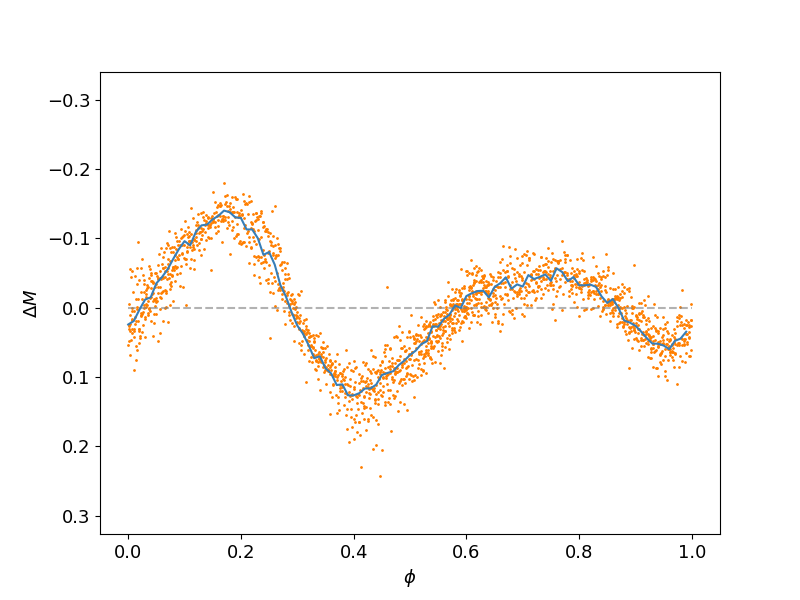
\includegraphics[width = \linewidth]{FastSolveAllCurve.png}
    \caption{A plot of all variances in the magnitude of Mitaka, $\Delta M$, in orange by phase, $\phi$, for a period of $P = 0.126$ days. The blue line is the best-fit lightcurve found from \textit{fastsolve.py}. Error too small to be seen}
    \label{fig:bestLC}
\end{figure}

The best-fit lightcurve resultant from folding the observed lightcurves is shown against the data from each night can be seen in \reffig{\ref{fig:bestLC}}, using $P_w = 0.1264707842$. The good agreement between the orange data points and blue best-fit curve show that the model is a good fit for the light curve of Mitaka.

\begin{figure*}\label{FastSolveAllEntire}
\centering
  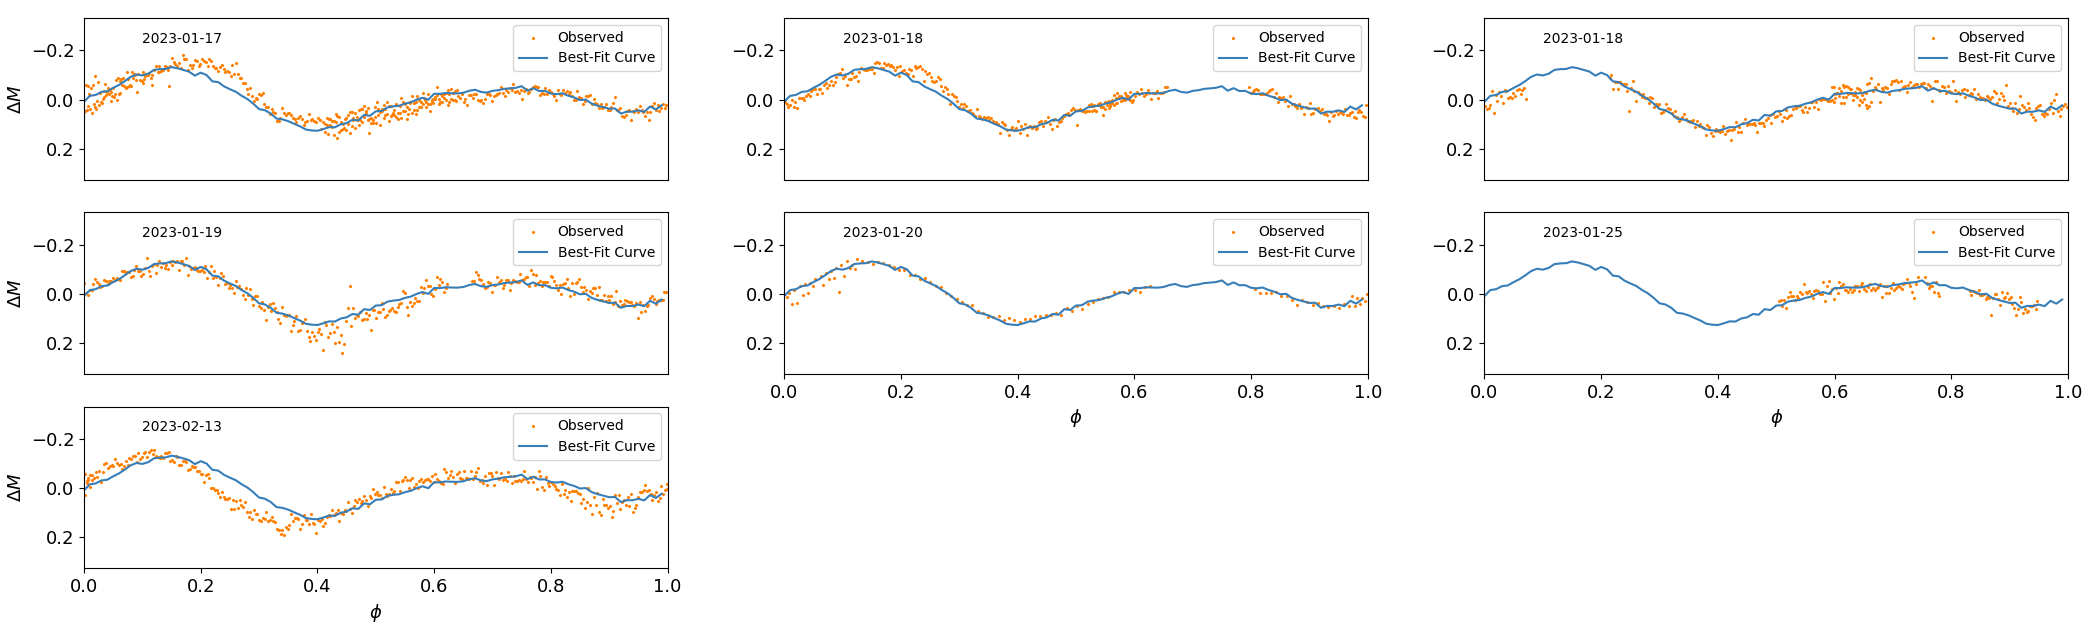
\includegraphics[width = \linewidth]{FastSolveAllEntire.png}
  \caption{A plot of variances in the magnitude of Mitaka in each data set,$\Delta M$, by phase ,$\phi$, for a period of $P = 0.126$ days. The blue line is the best-fit lightcurve found from \textit{fastsolve.py} using all data sets and the orange points are the folded observations at their corresponding phase. Error too small to be seen.}
\end{figure*}


\section{Making the model}
 
To make a model of the asteroid, the lightcurve will be analysed to make a convex hull that can be discretised into facets. For a more full description of this process, see \cite{ModelMaking}.

Firstly, the observed brightness, $\textbf{L}$, must be related to the parameters of the model $\textbf{g}$, which can either be the facets of a convex polyhedron or the coefficients of a spherical harmonic depending on the solving method, two of which will be discussed,
\begin{equation}\label{eqn:Landg}
    \textbf{L} = A\textbf{g}.
\end{equation}
$A$ is a matrix representing the scattering law, $S$, and albedo of the model, $\varpi$,
\begin{equation}\label{eqn:matrixA}
    A_{ij} = S_j(\mu^{(ij)}_\earth,\mu^{(ij)}_\astrosun) \varpi_j,
\end{equation}
where $\mu_k = E_K \cdot n$, with $E_k$ is the unit vector towards $k$ (the Sun of Earth), and a $j$ subscript denotes the scattering and albedo of the $j^{th}$ facet. 

The scattering function used is the  Lommel–Seeliger law,
\begin{equation}
    S = \frac{\mu_\earth \mu_\astrosun}{\mu_\earth + \mu_\astrosun}
\end{equation}

In order to find the best shape to represent the asteroid, a minimisation is set up to find the best-fit $\textbf{g}$,
\begin{equation}\label{eqn:chi2OfModel}
    \chi^2 = ||\textbf{L} - A\textbf{g}||^2,
\end{equation}
as this will minimise the difference in observed brightness $L$ and model brightness $A\textbf{g}$.

As $\textbf{g}$ is the representation of a physical quantity, say area, it must be positive. To achieve this $\textbf{g}$ is parameterised as an exponential,
\begin{equation}
    \label{eqn:parametariseg}
    g_j = e^{a_j},
\end{equation}where due to the exponential being positive, $a_j$ is an unconstrained parameter, which is more practical for computation. This has the side effect of making the minimisation of \refeq{\ref{eqn:chi2OfModel}} a non-linear problem.

\subsection{Smooth Method}\label{ssec:smoothMethod}

The initial model shape of the asteroid is formed via a curvature function $G(\vartheta, \psi)$, where $\vartheta, \psi$ are the spherical coordinates of the surface normal at some point on the model.
\begin{equation}\label{eqn:curveFunct}
    G(\vartheta, \psi) = \exp \Bigl(\sum\limits_{lm} a_{lm} Y^m_l(\vartheta, \psi)\Bigl) 
\end{equation}.
The observed brightness can then be expressed in terms $G$,
\begin{equation}\label{eqn:brightnessandG}
    L = \int \int_{A_+} SG(\vartheta, \psi) d\sigma,
\end{equation}
where the integration region $A_+$ is the Gaussian image sphere, and $d\sigma$ signifies integrating over the surface of $A_+$. The Gaussian image sphere $A_+$ is a sphere centred on an object, each point of which represents a unique normal vector direction on the object's surface.
By discretising $A_+$ into triangular facets of area $\Delta \sigma_j$ to approximate $d\sigma$, the integration can be performed as a sum over this discretised sphere such to find the area of the model facets, $g_j$, such,
\begin{equation}
    \label{eqn:gfromG}
    g_j = G(\vartheta_j, \psi_j) \Delta \sigma_j,
\end{equation}
where $\vartheta_j, \psi_j$ are the angular coordinates of the facet $\Delta \sigma_j$. With dense enough discretisation, the numerical error from this process is negligible.

Therefore, because the number of $a_{lm}$ is typically between 40 to 100 and \refeq{\ref{eqn:chi2OfModel}} is non-linear, \refeq{\ref{eqn:chi2OfModel}} is minimised using the Levenberg–Marquardt optimization scheme to find values of $a_{lm}$ so the model brightness best-fits $L$.

The initial model shape can be taken as a triaxial ellipsoid, the curvature function of which $G_e$ can be expressed using \textbf{Eq. \ref{eqn:curveFunct}}, with a chosen number of coefficients $a_{lm}$. After solving for $a_{lm}$, $G$ is then found using \refeq{\ref{eqn:curveFunct}}.

After $G$ is found it can be discretised via \refeq{\ref{eqn:gfromG}} into facets which can then be made into a convex bulk. Alternatively, this initial shape can be passed to a scheme that converges to a better solution when given a rough initial shape. 

\subsection{Polyhedral Scheme}\label{ssec:polyhedraScheme}

As surfaces of constant $\xsqrd$ in $\textbf{g}$-space are convex, only one possible $\textbf{g}$, such $g_j \ge 0 \text{ } \forall \text{ } j$, minimises
$\xsqrd$. Also, as the exponential is monotonic, only one $\textbf{a}$ corresponds to any $\textbf{g}$. Therefore, $\xsqrd$ is minimised one and only one $\textbf{a}$, thus there is one unique minimum $\xsqrd$. As well, due to the monotonic nature of the exponential, this will be the only minimum, meaning that despite the introduction of non-linearity with \refeq{\ref{eqn:parametariseg}} the smallest solution can still be found.

The number of parameters must be large ($\mathcal{O}(10^3)$) so the result is independent of the surface normal directions, $\xsqrd$ in \refeq{\ref{eqn:chi2OfModel}} then minimised using the conjugate gradient method \textbf{\cite{conjugateGradMethod}}, in order to find the facet areas $\textbf{g}$.
    
After this, the Minkowski procedure can be used with the know facet areas $g$ in order to find the facet vertices. 
If we have the facet areas $g$ and surface normals, the reconstruction of the polyhedron can be expressed as a maximisation problem with the volume of the polyhedron $V(\textbf{l})$ being solved for, where $\textbf{l}$ is the distance from the facets to the origin. The constraint for this is that the inner-product $\langle \textbf{l},\textbf{g} \rangle$ is constant, and the volume $V(\textbf{l})$,
\begin{equation}
    \label{eqn:polyhedraVol}
    V(\textbf{l}) = \sum\limits_{j=1}^n l_j A_j(\textbf{l}),
\end{equation} where $A_j(\textbf{l})$ is the area of facet $j$ calculated from $\textbf{l}$.

The gradient of this volume is simply $\textbf{A}$ and its projection onto the constraint plane is,
\begin{equation}
    \label{eqn:APOnConstraint}
    \textbf{f} = \textbf{A} - \frac{\langle \textbf{A}, \textbf{g} \rangle}{\langle \textbf{g},\textbf{g} \rangle} \textbf{g}.
\end{equation} Using this projected gradient ensured that any iterations made using the gradient fulfil the constraint automatically. 
Using the dual transform (DT), which maps planes to points and vice versa, the facets calculated can be used to find the vertices of the polyhedron. The DT takes a plane with surface unit normal $\hat{\textbf{n}}$ and distance from origin $l$ into a point of radius vector, $\textbf{r}$,
\begin{equation}
    \label{eqn:radiusVector}
    \textbf{r} = \frac{\hat{\textbf{n}}}{l}.
\end{equation}
Importantly the adjacency of facets and vertices is preserved, adjacent facets are mapped to connected vertices, the vertices of a facet become connected facets, etc.

So, after the facets are found, the DT is performed and the convex hull of the dual vertices (which represent facets in real space) is found, where the convex hull is the envelope around a set of points such each point can be connected to any other with a straight line without leaving the envelope. The facets of the dual convex hull are then transformed into vertices in real space. This then completes the construction of a convex polyhedron corresponding to $\textbf{l}$, and $A_j(\textbf{l})$ is found via simple geometry using the surface normals.

\begin{figure}
    \centering
    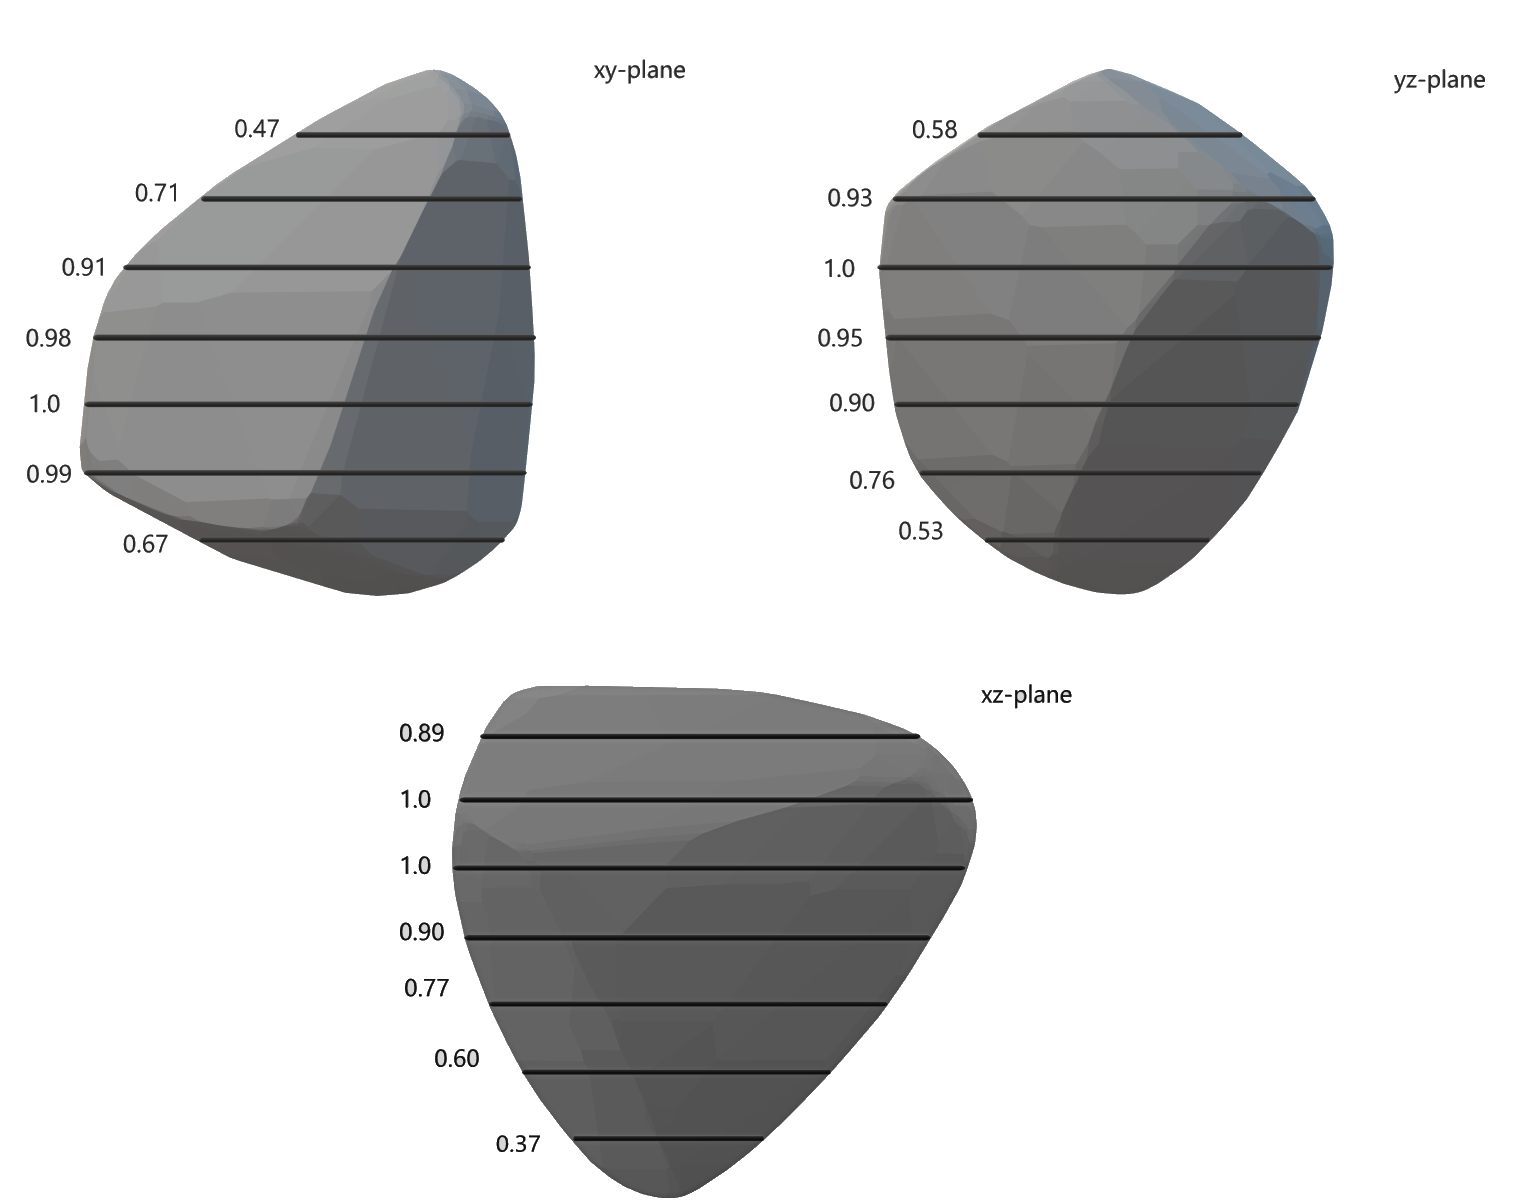
\includegraphics[width = \linewidth]{allProj.png}
    \caption{The projection of Mitaka in the xy, xz, and yz-planes. The Ratio of diameter to maximal diameter are shown for several points on projection.}
    \label{fig:allProj}
\end{figure}

\begin{figure*}
    \centering
    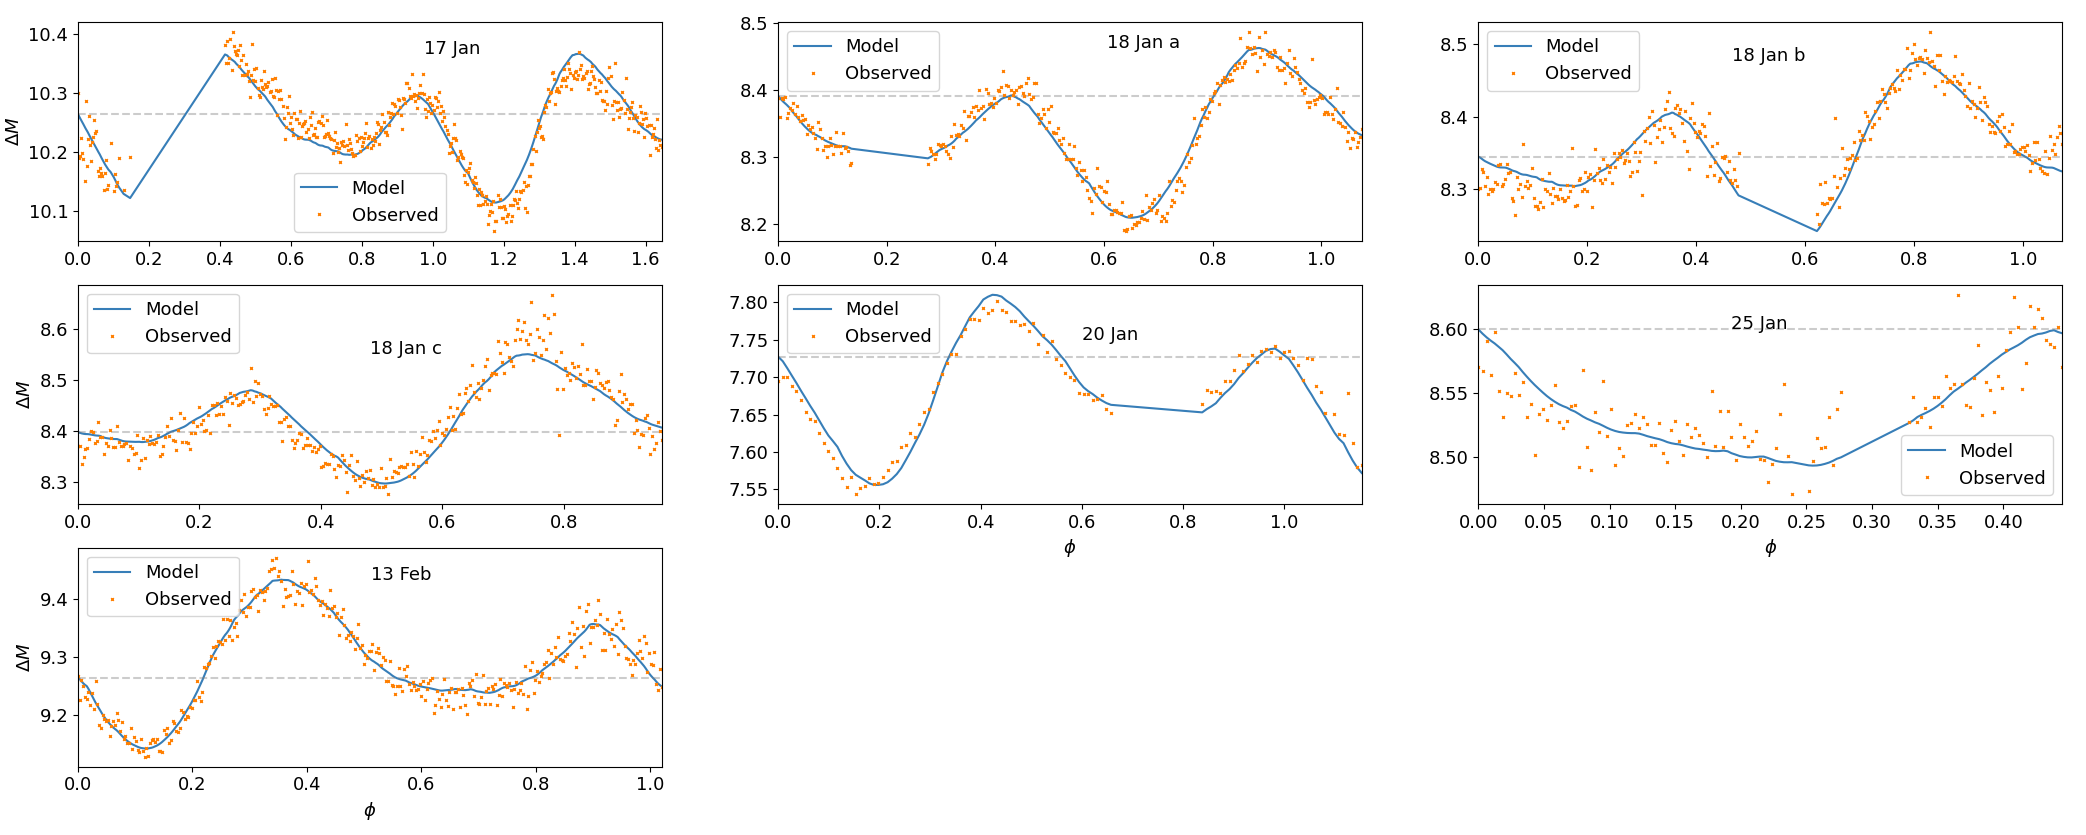
\includegraphics[width = \linewidth]{compareLC.png}
    \caption{The relative observed magnitude of Mitaka and of the model, $M_0 = 20$, in order to see how well the model agrees with the observations. The straight blue lines and the gap in orange points are due to the removal of erroneous data due to Mitaka transiting stars. Errors too small to be seen.}
    \label{fig:compareLCS}
\end{figure*}


\section{Finding the Bulk Quantities}\label{ssec:findVM}


An asteroid will have some portion of the solar luminosity, $L_\astrosun$ incident on it according to the cross-sectional area facing the sun, $A_{a}$,
\begin{equation}\label{eqn:fluxAsteroid}
    f_{a} = \frac{ L_\astrosun A_{a}}{4\pi r^2_{\astrosun,a}},
\end{equation}
where $f_a$ is the flux incident on the asteroid and the denominator is a term describing the inverse square law for luminosity propagating from/as a sphere.

After this the asteroid will reflect a proportion of this flux to Earth, $f_\earth$ according to its albedo, $\varpi_{a}$, such
\begin{equation}\label{eqn:fluxEarth}
    f_\earth = \frac{f_{a} \varpi_{a}}{2r^2_{\earth,a}},
\end{equation}
where the denominator is the inverse square law for luminosity propagating from/as, and $f_\earth$ is what flux incident on Earth. $f_\earth$, therefore, is calculated via the magnitude of the asteroid in the collected images. 

But unlike solving for variations in the brightness over time absolute zero-point (meaning the magnitude of a 1 count per second object), $M_0 \equiv 0$, is needed to calculate physical properties like area from flux. This means $f_\earth$ will be compared with the flux of Vega, $f_v$, which has magnitude, $M_v$, set to be $0$ in order to find $A_a$.

The ratio of flux between two objects can be expressed in terms of their magnitudes,
\begin{equation}\label{eqn:fluxRatio}
    \frac{f_{\earth}}{f_{*}} = 10^{\frac{M_{a} - M_{*}}{-2.5}},
\end{equation}
which is a rearrangement of \textbf{Eq. \ref{eqn:Mag}}. 
$M_v \equiv 0$ and Vega has known flux $f^v_{5556} = 3.46\times10^{-9} \pm	2.422\times10^{-11}
ergs s^{-1} cm^{-2} \AA^{-1}$ at $5556 \AA$ \textbf{\cite{VegaMag0}}, which becomes $f_v = 1.92238\times10^{-8}\pm 1.34566\times10^{-10} J s^{-1} m^{-2}$ in SI units in the clear band. 
So, the flux incident on earth from an asteroid is
\begin{equation}
    \label{eqn:fluxOnEarth}
    f_\earth = 10^{-0.4M_a} \cdot 1.92238\times10^{-8}
\end{equation}


Now the distances $r_\earth,a$ and $r_\astrosun,a$ must be found. A triangle can be constructed between the Earth, Sun, and the asteroid. The semi-major axis of the asteroid orbit $a_a$ can be taken as $r_{\astrosun,a}$, $r_{\astrosun,\earth} \equiv 1AU$. But, to find $r_{\earth, a}$ the Sun-Target-Earth angle, $STE$, and the Sun-Earth-Target angle, $SET$, are used to calculate the Earth-Sun-Target angle $\EST = \pi - SET - STE$, then using the cosine rule with the known sides,
\begin{equation} \label{eqn:cosRule}
    r_{\earth,a}^2 = r_{\astrosun, a}^2 + r_{\astrosun, \earth}^2 - 2 r_{\astrosun,a} r_{\astrosun,\earth}\cos{(\angle_{\earth\astrosun a})}.
\end{equation}Note this makes no assumption of the angles of the EST triangle, and is general to any celestial configuration.  


Substituting \textbf{Eq. \ref{eqn:fluxAsteroid}} into \textbf{Eq. \ref{eqn:fluxEarth}} and rearranging for $A_{a}$ it can be found,
\begin{equation}\label{eqn:areaAsteroid}
    A_{a} = \frac{f_\earth 8 \pi^2 r^2_{\astrosun,a} r^2_{\earth, a}}{L_\astrosun \varpi_{a}},
\end{equation}
using the previously calculated  $f_\earth$ and $r_{\earth,a}$.

If the area of two faces of the asteroid are calculated $A^a_i$, then the phase difference between those faces $\Delta \phi$ gives the angle between them $\theta = 2\pi \Delta \phi$. From this, a third face can be constructed to form a parallelogram-faced prism to approximate the asteroid's volume $V_a$.
This is done by first taking one of the faces to be a square of area $A^a_1$ and side length $l_1 = \sqrt{A^a_1}$. Then another face will be a rectangle of area $A^a_2$ and side lengths $l_1$ and $l_2 = A^a_2/l_1$. These faces have an angle of $\theta$ between their shared edge, resulting in a third parallelogram face with area,

\begin{equation}\label{eqn:Aa3}
    \begin{split}
    A^a_3  &= l_1 l_2 \sin{(\theta)}, \theta \leq \pi, \\
            &= l_1 l_2 \sin{(\pi - \theta)}, \theta > \pi, \\
    \end{split}
\end{equation}

The total approximate volume of the asteroid is then the volume of the constructed parallelogram-faced prism. 
 \begin{equation}
     V_a = l_1 A^a_3.
 \end{equation}

From here the density of the asteroid, $\rho_a$, can be used to approximate the asteroid mass, $m_a$, with $m_a = \rho_a V_a$, and the composition of the asteroid by comparison to average material densities in asteroids, seen in \textbf{Tab \ref{tab:compTab}}.

Mitaka was analysed in two images from 19 Jan taken $0.814hr$ apart, equivalent to a phase difference $\Delta \phi \approx 0.27$. In these images, Mitaka had counts $S^w_\alpha = 50433 \pm 6.051$ and $M^w_\Omega = 12268 \pm 7.3449$ respectively. Each image has its own absolute zero-point $M_0^\alpha = 25.924 \pm 0.007$ and $M_0^\Omega = 24.447 \pm 0.014$ calculated by a local python script called \textit{find \textunderscore zeropint.py}.Using \textbf{Eq. \ref{eqn:Mag}} with these $M_0$ and $S$ values the magnitudes are found, $M_{\alpha} = 14.167 \pm 0.007$ and $M_\Omega = 14.026 \pm 0.01$. 

Mitaka has a semi-major axis about the sun of $a_w = 2.201288900683571$, and $r_{\astrosun,w}$ will be taken as this. The find $r_{\earth,w}$, the necessary angles are found from the JPL ephemeris database \cite{jplEphAngle} for the time of each image (~04:37 for $\alpha$, ~05:26 for $\Omega$), $STE_\alpha = 8.9216$, $SET_\alpha = 160.1291$, $STE_\Omega = 8.9097$, and $SET_\Omega = 160.0939$. Using These angles and distances it can be found $r_{\earth,w}^\alpha = 1.52324112 \pm 1\times10^{-10}AU$ and $r_{\earth,w}^\Omega = 4 \pm 3AU$


So now with $r_{\earth,w}$, $r_{\astrosun,w}$, and $f_\earth$ calculated using magnitude with \refeq{\ref{eqn:fluxOnEarth}}, with $L_\astrosun = 3.842\times10^{26} Js^{-1}$
\textbf{\cite{LSol}} and the albedo of Mitaka $\varpi_w = 0.15$. The areas then from both images are found using \textbf{Eq. \ref{eqn:areaAsteroid}}, $A_\alpha=(300 \pm 60)\times10^6 m^2$ and $A_\Omega = (500\pm 600)\times10^6 m^2$. This gives side lengths of $l^w_1=18000
 \pm 2000 m$ and $l^w_2 = 30000
 \pm 30000 m$. The phase difference of these faces is $\Delta \phi \approx 0.268$ which means an angle $\theta = 2\pi \Delta \phi = 1.455$. Therefore the area of the parallelogram face is $A^{w_3} = (5 \pm 6)\times10^8 m^2$, with finally total area $A_w = 2000 \pm 3000 Km^2$ and volume $V_w = 8000 \pm 13100 Km^3$.


The average density of a set of S-type asteroids in \textbf{\cite{STypeDenstiy}} is $\rho_S = 3000 \pm 900 Kg m^{-3}$, which can be used to calculate an estimated mass of Mitaka of $m_w = (2 \pm 4)\times10^{13} Kg$ and a composition shown in table \reftab{\ref{tab:compTab}} derived from the average fractional masses of minerals $Z$ found using spectroscopy of S-type asteroids in \textbf{\cite{sComp}}.

\begin{table}[]
    \centering
    \begin{tabular}{c|c|c}
         Material & $Z$ [\%] & Mass in Mitaka [Kg$\times10^{12}$] \\ \hline
         clinopyroxene  & $9.4 \pm 0.8$    & $2 \pm 4$\\
         orthopyroxene  & $12 \pm 2$        & $3 \pm 5$\\
         olivine        & $32 \pm 2$        & $8 \pm 10$\\
         Fe,Ni          & $30 \pm 3$        & $7 \pm 10$\\
         Troilite        & $16 \pm 1$        & $4 \pm 6$\\
         Total          & $100 \pm 9$           & $24 \pm 40$\\
    \end{tabular}
    \caption{A table showing the average fractional mass $Z$ of minerals in S-type asteroids derived from \cite{sComp}} and the mass of materials calculated to be in Mitaka. 
    \label{tab:compTab}
\end{table}



\section{Discussion}\label{sec:discussion}
First will be discussed the accuracy and error from observation and photometry of Mitaka. The minimum seeing achieved in observations was $3"$, and weather during observations was mostly clear. The best $S/N$ was $~360$, shown in \reffig{\ref{fig:SMAPlot}}, meaning the noise is $360$ times smaller than the signal observed. Therefore the observations can be said to be measuring the brightness of Mitaka quite accurately. Looking at \reffig{\ref{fig:mask}} the difference between the masks from both stars are do not vary much for 17 Jan, and the same was true for the masks from all other nights. This validates that the mask used will be able to accurately account for disturbances in the measured brightness of Mitaka.

Now looking at the construction of the model, firstly in \reffig{\ref{fig:bestLC}} the best-fit curve passes through the observation points very well, which is indicative that the lightcurve folding resulted in a good fit, and so the period of this curve $P_w = 0.1264707842 \pm 1\times10^{-10}days$ is an accurate period for Mitaka. The error in $P_s$ being of order $\E{-10} days$ is also a good indication that the period has been solved to high accuracy. However finding the best-fit curve is a numerical method, it uses bins and a set of periods in order to find the period, which means by raising the number of bins the accuracy can be rendered to arbitrarily high decimal places. However, the jackknifing process used to find the variance which is then used to calculate the error in $P_w$.As an arbitrarily high accuracy for each point will not necessarily mean a greater precision between all of them, meaning the error reported on $P_w$, $\err{P_w}$, can not be made arbitrarily low by using a large number of bins. This means that $\err{P_w}$ is still indicative of an actual variance in solving for $P_w$ not numerical error. 

Also looking at \reffig{\ref{fig:findP}}, three distinct faces can be inferred. There are two lower magnitude faces at $\phi = 0.17, 0.75$, the earlier being brighter than the other, and a higher magnitude face at $\phi = 0.4$. This implies two larger faces that have a smaller face in between, with respect to the direction vector of Mitaka to Earth $\hat{\textbf{r}}_{w,\earth}$. 

Reviewing the model, the lightcurve of the model in \reffig{\ref{fig:compareLCS}} passes through the observed points for each night. This shows that the model shape is a valid model of Mitaka as it clearly scatters light in the same way as Mitaka. 

The model itself, seen in \reffig{\ref{fig:allProj}} shows that Mitaka has many large, flat areas. Most of these large, flat surfaces in the xy-plane are also around half the width of that entire projection, corresponding to $~18Km$ using $r_w = (4V_w/3)^{1/3}$. This means there is a large, flat area on which spacecraft could land, meaning that Mitaka would be a good candidate for mining in terms of being able to set up equipment.  
The shape of Mitaka is roughly a triangular pyramid on top of a cone, as the top is two connected faces that slope down into meeting a body that tapers in gently toward to tip. This shape is useful for mining for several reasons. 
One is that as Mitaka has sloped surfaces on its conoid part different layers of it can be accessed by moving across and then mining in rather than having to mine through the entire distance. This makes resources easier to collect as less energy, time, and mining is needed to get to them in comparison to if Mitaka was more isomorphic in shape.
The natural ramp this sloping creates is also useful for moving around Mitaka as instead of having to create complicated machinery to traverse harsh inclines and drops, a simple wheeled or tracked vehicle could drive on the surface in order to get to any point on Mitaka. 
Both of these features reduce the energy needs and the mechanical complexity of the equipment that would be needed to mine Mitaka, which overall makes the endeavour more technically and financially viable. 

The conoidal shape of Mitaka also means the centre of gravity (COG) of Mitaka will not fluctuate as may happen with asteroids of more irregular shape. Landing on the broader top of Mitaka would mean mining would go toward the tip. As the COG of a cone is a quarter of the height up from the base, and mining Mitaka towards the tip would preserve its conoidal shape, the dynamics of the shape and COG of Mitaka would not vary greatly, meaning a mining system would theoretically not need the same robustness as an asteroid who's COG would move drastically as it was mined, and the mass distribution changed. 

However, it must not be forgotten that the model created is convex in nature, and can not model surface imperfections. This includes craters, boulders, local steep inclines, etc. The risk to equipment from this is that if a craft is expecting a landing zone to be a certain way, it will be braced as such. So if the landing site is, or is near, a crater then the craft may not have the capability to land safely at the greater depth or may impact the ridge and be damaged in the process. The curved nature of the crater may also mean the landing equipment may not be able to anchor into the surface properly if it was meant for a flat surface. A boulder could also be an issue, as if a craft lands near to one and disturbs it, this could cause the boulder to move onto the craft, possibly glancing the hull or maybe crushing it all together. This means that the detection of these features is vitally important, which sadly this modelling solution can not achieve.
Also, these craters and boulders may be indicative of the more valuable material available on Mitaka. A boulder could be resultant of material from inside Mitaka that has withstood erosion, meaning it would be the more durable metallic material, such as Fe-Ni, available on Mitaka. Craters may also hold more valuable material as they will contain material from other asteroids and also provide shelter for elements that would evaporate off of Mitaka if exposed to the Sun. Therefore not being able to find these features would mean not detecting areas of possible greater mining potential.

As for the composition of Mitaka, it is clearly very rich in Fe-Ni, being $~30\%$ of its composition resulting in an approximate mass of $7\times10^{12} Kg$. This material would be useful to any mining operation on Mitaka and would have plenty to send to Earth as well. On Mitaka, the Fe-Ni could be used to build new craft to be used in mining. If say Mitaka was the first lading of a mining probe in what was to become a fleet, then the abundance of metallic material in Mitaka would allow the construction on many 100s of other mining craft which could then be sent to other local asteroids. If also humans were part of the mining operation, then the Fe-Ni could be used to create radiation shielding for human workers so as to not expose them directly to the unattenuated rays of the Sun.
Mitaka also contains $~5\E{12} Kg$ of pyroxene, which is useful in space for many uses. Pyroxene is commonly crushed into rock for use in construction, meaning that it could be used in space to build strong buildings. 
Pyroxenes can also contain Lithium \cite{LiInProx}. This is an important element for making batteries, opening up the possibility of creating new electronic machinery in space from Fe-Ni power by Li batteries powered by solar panels, possibly also created by the silicon on Mitaka. Lithium is also useful in machinery as it can be used in making grease for the joints in the machinery, which is important for the longevity of the mining equipment.
Lithium is also used as a flux in the processing of silica, which will be important as Mitaka being an S-type asteroid will contain a lot of silicon. 
Mitaka also contains olivine, a magnesium-iron silicate.

Troilite is a simple iron sulphide mineral FeS more common in meteorites than native on Earth. There to be able to mine it in large amounts, Mitaka containing $4\E{12}$, would open up the opportunity to study its properties and experiment with possible on and off-world uses. 

However, the large amount of error on these values can not be ignored. While Mitaka is an S-type asteroid and will contain these minerals in large amounts, the specific amounts calculated are clearly not a reliable point of reference. Mitaka will contain the minerals specified, it is an S-type asteroid and would not be designated so if it did not. As well, the albedo of Mitaka $\varpi_w = 0.15 \pm 0.03$ which is comparable to the albedos of other S-types \cite{mitakaAlbedo}, so it is likely to contain the same minerals, at least on the surface. However, the actual amount can clearly not be specified well by comparison to other asteroids. The error present in the percent composition is at minimum $\pm 0.8\%$ which corresponds to an uncertainty of $8\E{11} Kg$ which is a lot of material, and the rest of the minerals only have more uncertainty. As well, actually then calculating the composition of Mitaka carries the error from calculating the mass, which is very large and also is clearly erroneously large due to the use of $\rsm = a_w$. This overall then leads to these errors combining into an error in the mineral masses that are larger than the mass of the mineral itself.

Finally, Mitaka has a literature diameter of $d^w_{Lit} = 15.957 \pm 1.596$ \cite{mitakaAlbedo}. Assuming a spherical shape to first order this corresponds to a volume of $V^w_{Lit} = 2.12742\E{12} m^3$ which is $~3.77$ times smaller than the calculated value in \textbf{Sec.\ref{ssec:findVM}}. Mitaka being found to be larger than in literature implies that the observations were measured to be brighter than would be expected. As Mitaka appears too bright, this is not the fault of not performing differential photometry on the images used to find the volume of Mitaka, as any disruption would make the Mitaka appear dimmer. This leads to the most likely cause of the discrepancy arising from the use of $\rsm = a_w$. As the distance from Earth to Mitaka $r_{\earth,w}$ was found using the semi-major axis of Mitaka $a_w$ as the Mitaka-Sun distance $r_{\astrosun,w}$, this does not account for the eccentricity of the orbit of Mitaka of $e_w = 0.19577183 \pm	1.12\E{-8}$. As this means the orbit of Mitaka is not circular, the use of $a_w = r_{\astrosun,w}$ will cause Mitaka to seem too bright if Mitaka is actually closer to the Earth, or dimmer if it is further. This naive assumption then can cause a large variation in the calculated area, volume, and mass of Mitaka due to the large possible differences between $a_w$ and $\rsm$, compounded by the relation $V_w \propto \rsm^4$, where the quartic term deriving from how $\rem^2 \propto \rsm^2$ \refeq{\ref{eqn:cosRule}} and $A_w \propto \rsm^2 \rem^2$ \refeq{\ref{eqn:areaAsteroid}}. Therefore, as Mitaka is more massive than expected, it can be assumed that Mitaka is closer to Earth than the use of $\rsm = a_w$ would suggest. This error also carries forward into the errors of the composite material in Mitaka, which is why the errors are of the same order as the actual amounts, as discussed previously. In future work then, if the distance between the asteroid being assessed, Earth, and the Sun was calculated more accurately at the time of observation, this method of calculating the mass and composition of the asteroid may yet be found to be useful, through this, of course, must be offset by the usefulness of this method being the ease of implementation with any standard astronomical equipment.  

\section{Conclusions}\label{sec:cnclusion}
The observations of Mitaka are good and are unlikely to be a source of significant error. A signal-to-noise ratio $S/N$ of $~360$ means that the signal is much larger than the noise which indicates the error directly from aperture photometry is small. The differential photometry is also accurate as the masks generated from two different calibration stars were very close, so have corrected for atmospheric conditions the same way, as expected. This overall means that the photometric measurements used in the modelling of Mitaka are good.

The lightcurve folding process has also been proven effective in finding the period of Mitaka. The lightcurve generated from \textit{fastsolve.py} by minimising the spread of magnitude $M$ within a specified range of phase $\phi$ agrees very well with the observed lightcurve, shown in \reffig{\ref{fig:findP}} by the fitted curve passing through the observed points, and its shape matching the shape the points form. Therefore this method of observing an asteroid as it rotates and modelling a curve with a period in order to find out the period of the asteroid is effective in accurately finding the period of the asteroid.

Once the period of Mitaka is found and a lightcurve is fit to the data a model of the asteroid can be created by describing a convex model in terms of facets with vector surface normals, and minimising the difference in the model lightcurve and that of Mitaka. The model provides an understanding of the overall hull shape of Mitaka. The lightcurve generated from the model passes through the lightcurves observed, \reffig{\ref{fig:compareLCS}}, which is a good indication the shape generated is reflective of Mitaka. 
However there are limitations in the modelling as the shape convex is a convex hull, meaning surface characteristics such as craters and outcroppings (e.g. boulders) are not able to be seen, their effects adding to the formation of flat facets. This means while the appropriateness of the shape for mining can be discussed in general terms: considering centres of gravity; how Mitaka can be traversed; and where on Mitaka may have enough landing and building area; the planning of specific landing areas and surveying for the locations of concentrations of specific minerals is not possible. 

The next step in assessing the prospect of mining Mitaka then was composition, which was found via comparison to other S-type asteroids. Unfortunately, the amount of calculation needed allowed many errors to combine so that the findings are not as useful as the model of Mitaka.
The areas of the faces of Mitaka being calculated with  raw data, not adjusted with differential photomerty, means that Mitaka will most likely appear dimmer in the data than in reality, especially likely as the observations were made in Durham. This effect however is not as significant as the use of the semi-major axis of Mitaka $a_w$ as its distance from the Sun $\rsm$. As $A_w \propto \rsm^4$ having an erroneous value for $\rsm$ causes significant discrepancy from an accurate value of $A_w$, and as the approximated volume is over triple what would be expected, this is the most likely cause of the discrepancy.

This then will carry forward into the error on the components of Mitaka. The percent compositions already had error that may change the amount of material by terrakilogrammes, but combining this with the error on the mass of Mitaka causes an error larger than the mass of material, which means the estimations of the amounts of each material is at best an indication of which are more common than other, which is what comparing percent composition already achieved with far less work.

Therefore overall, the technique of measuring the variation of the brightness of an asteroid can allow the accurate calculation of its period and even be used in combination with mathematical machinery in advanced geometry to find its approximate convex shape. But, the inability to find the finer details of the surface of the asteroid such as craters and out-croppings means that for mining prospects this technique will most likely be limited to preliminary observations in order to gauge the appropriateness of an asteroids shape for movement of materials and craft, and the stability of the centre of gravity as material is removed. 



\bibliography{refs.bib}

\clearpage

\section*{Observation Log}

\begin{table}[h]
    \centering
    \begin{tabular}{|l|l|l|l|l|l|}\hline
        Date & Time (UTC) & Telescope & Band & Notes \\ \hline
        17/01/2023 &  18:41 - 23:41 & Draco-2 & C & Except 19:36 - 19:56, no visible stars after 23:40. \\
        18/01/2023 & 20:33 - 06:40 & Draco-2 & C & \\
        20/01/2023 & 19:05 - 23:02 & East-16 & C & No visible stars between 19:23 - 19:25, and after 22:59. \\
        25/01/2023 & 19:29 - 20:50 & Draco-2 & C & \\
        13/02/2023 & 20:24 - 23:43 & Draco-2 & C & \\ \hline
    \end{tabular}
    \caption{Table of Observations through 17/01/2023 to 13/02/2023}
    \label{tab:obsTable}
\end{table}

\clearpage

\section*{Error Appendix}
Most errors $\alpha$ are calculated with two methods. Firstly by adding errors in quadrature,
\begin{equation}
    \err{V} = V\sqrt{\sum\limits_i{(\frac{\err_{C_i}}{C_i})}},
\end{equation}where $V$ is the value being calculated and $C_i$ are the values used in its calculation.
Or secondly by using the functional approach,
\begin{equation}
    \err{V} = |f(C_0 + \err{C_0}, ... , C_N + \err{C_N}) - f(C_0, ... , C_N)|
\end{equation}

\subsection{Jackknifing}\label{ssec:jackknifing}
Some errors are calculated via Jackknife resampling, or "jackknifing", a statistical method used to estimate the accuracy of a value $V$ calculated from a data-set $D$. This is done via resampling $D$ excluding one datum $x_i$, repeated to exclude each datum once. This results in $N$ data-sets ${D_i}$, where N is the number of data in $D$. Then the value $V_i$ is calculated again using each $D_i$, and may differ from, $V$. 
In the case many data-sets $\{D\}$ are used in the calculation of the value, an entire data-sets $D_i$ is excluded in jackknifing.  
The standard error of the value, $\err{V}$ is then similar to the normal standard error, calculated via the values from jackknifing
\begin{equation} \label{eqn:errFromJK}
    \err{V} = \sqrt{\frac{(n-1)}{n} \sum\limits_{i=1}^{N} (V_{i} - \overline{V_J})^2},
\end{equation}
where $\overline{V_J}$ the mean of the jackknife values,
\begin{equation}
   \overline{V_J} = \frac{1}{n} \sum\limits_{i = 0}^N  V_i
\end{equation}

The error in $P_w$ was calculated by finding the period again, but excluding a single night, until all nights have been excluded. The jackknifed periods can be seen in \reftab{\ref{tab:jackP}}.

\begin{table}[h]
    \centering
    \begin{tabular}{c|c}
         data excluded & period $P_J$  \\\hline
         none       & 0.126475 \\
         17 Jan     & 0.12647078416666666 \\
         18 Jan a   & 0.12647078416666666 \\
         18 Jan b   & 0.12647078416666666 \\
         18 Jan c   & 0.12647078416666666\\
         20 Jan     & 0.12647078416666666\\
         25 Jan     & 0.12646656833333333\\
         13 Feb     & 0.12644548916666667\\
    \end{tabular}
    \caption{A table showing the periods $P_J$ found via excluding a set of observations when calculating $P$ for the jackknifing process, used to find the error in $P_w$.}
    \label{tab:jackP}
\end{table}

These values then, using \refeq{\ref{eqn:errFromJK}}, give an error on the period of $\err{P_w} = 1\times10^{-10}days$.

\err{$a_w$} was given in the JPL small body database as $4.0712\times10^{-9}AU$

\err{$\varpi_w$} was given in \cite{mitakaAlbedo} as $0.03$

\err{$f_v$} was given in \cite{VegaMag0} as $2.422\times10^{-11} ergs s^{-1} cm^{-2} \AA^{-1}$

\err{$S^w_\alpha$} and \err{$S^w_\Omega$} were given by the GAIA imaging software as $6.051$ and $7.24449$ respectively.

\err{$M_0^\alpha$} and \err{$M_0^\Omega$} were found using \textit{find \textunderscore zeropint.py} and were $0.007$ and $24.447$ respectively.

\err{$M_\alpha$} and \err{$M_Omega$} were found using the functional approach using \refeq{\ref{eqn:Mag}}, and were $0.007$ and $0.001$ respectively. 

\err{$\rsm$} was taken as \err{$a_w$} which was $4.0712\times10^{-9}AU$ as above.

\err{$\rem^\alpha$} and \err{$\rem^\Omega$} were calculated with the functional approach and \refeq{\ref{eqn:cosRule}} and were  $1\times10^{-10}AU$ and $3AU$ respectively.

\err{$L_\astrosun$} was found in \cite{LSol} and was $10^{26} Js^{-1}$.

\err{$A_\alpha$} and \err{$A_\Omega$} were found via the functional approach with \refeq{\ref{eqn:areaAsteroid}} and were $6\E{7} m^2$ and $6\E{8}$ respectively.

\err{$l_1$} was found using the functional approach with $l_1 = \sqrt{A_1}$ and was $2000m$

\err{$l_2$} was found by adding error in quadrature where $l_2 = A_\Omega/l_1$ and was $30000m$

\err{$A_3$} was found using the functional method with \refeq{\ref{eqn:Aa3}} and was $6\E{8} m^2$

\err{$A_w$} was found via the functional method with $A_w = 2(A^w_\alpha + A^w_\Omega + A^w_3)$ and was $3\E{9} m^2$

\err{$V_w$} was found via the functional method with \refeq{\ref{eqn:polyhedraVol}} and was $1\E{13} m^2$

\err{$\rho_S$} was found as the standard error of the set of S-type densities in \cite{STypeDenstiy}, and was $900 Kg m^{-3}$

\err{$Z$} are S-type asteroids was given in \cite{sComp} and were 

The error in the mass of each mineral on Mitaka was found by adding error in quadrature using $m_{mineral} = m_w Z$ 




\clearpage

\onecolumngrid %Puts Summary into single column

\section*{Scientific Summary for a General Audience}

Asteroid mining may be the future of gaining more resources either to use on Earth or in space to create a Human civilisation amongst the stars. Bringing resources back to Earth would effect the price of what is brought back greatly due to the new massive influx, but the use of the minerals in space is an even more exciting idea. These asteroids will obviously need to be screened to assess which asteroids are good candidates. Due to the cost and complexity of high-resolution images to see what asteroids look like, a simpler approach can be found this will allow asteroids to be screened with higher efficiency would be very useful for finding asteroids to mine. As asteroids are most commonly not spherical, and they spin like Earth, different parts of the asteroid with different sizes will face Earth at different times. The changes in brightness through time create a curve called a lightcurve (LC), and by analysing this LC a model of an asteroid can be constructed to assess if the shape of the asteroid is suitable for mining. Then the mass of minerals in the asteroid can be approximated by comparison to other asteroids of its class, and calculating its volume from the flux of the asteroid incident on Earth.


\end{document}